%---------- COURSE INFORMATION ------------------------
\newcommand{\course}{CS 490-01}
\newcommand{\coursetitle}{Senior Seminar}
\newcommand{\courseloc}{N/A}
\newcommand{\coursetime}{N/A}
\newcommand{\coursedesc}{Computer science topics selected according to the needs of the students.}

\newcommand{\coursesec}{01}
\newcommand{\coursecredithours}{3}
\newcommand{\courseprereq}{Departmental approval.}
\newcommand{\coursedelmethod}{Individual instruction}

\newcommand{\courseobjectives}{\item Explain the role of operating systems for software development.
	\item Develop an embedded simple operating system to handle simple signal based tasks.
	\item Explain various system architectures and how the operating systems manage both the hardware and software.
}

\newcommand{\coursetopics}{\item Instruction set architectures
	\item Memory
	\item I/O and storage
	\item Ebedded systems
	\item OS performance and metrics
	\item OS data structures
}
\newcommand{\coursegrades}{Subject Exams (2 exams @ 20\% each)\dotfillsmall 40\% \\
		Project Work\dotfillsmall 30\% \\
		Final Project\dotfillsmall 30\% }
\newcommand{\coursetext}{
	\adjustbox{valign=c}{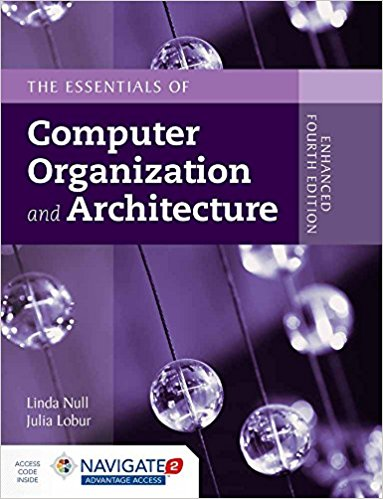
\includegraphics[width=1in]{img/cs490}} & \hangindent .4in \textbf{Textbook:} Null, L., Lobur, J. (2015). Essentials of Computer Organization and Architecture (4th edition). Jones \& Bartlett Learning. ISBN-10: 128407448X, ISBN-13: 978-1284074482. \\
	%& \hangindent .4in Simulation Software: SAM 365 \& 2016 Assessments, Trainings, and Projects with MindTap Reader.
}